
\chapter{Heuristické metody výuky}

Principem heuristických metod výuky je postavení žáka před problémovou situaci, kterou má vyřešit.
Situace by měli podněcovat žáka k překonávání těžkostí a vzbuzovat touhu po poznání. 
Heuristické metody vedou k osvojení poznatků skrze tvořivou činnost žáků, vymýšlení nového řešení na 
základě již známých znalostí.\cite{vanecek2016,zormanova2012}\\

Aplikace heuristických metod může mít v praxi různé formy: heuristický rozhovor, heuristický pokus, 
řešení úloh, verifikace tvrzení, řešení technických problémů a další. \cite{vanecek2016}. Heuristická 
výuka má poměrně dlouho tradici. V oblasti chemie byl jejím velkým zastáncem britský organický chemik 
Henry Edward Armstrong, který žil v letech  1848 -- 1937).\cite{armstrong_britannica, armstrong_heuristic_method} \\

Heuristická výuka vyžaduje určité specifické předpoklady jak pro pedagoga a žáky tak pro téma hodiny. 
Učební téma musí být dobře uchopené a musí být provedena vhodná didaktická transformace učiva. Ačkoliv 
to nemusí být zřejmé, většina témat jsou vhodná k heuristickém metodám, méně vhodná mohou být například 
abstraktní témata, ale obecně lze tyto metody aplikovat na libovolné učivo. \cite{kropac2006, zieleniecova2012} 
S dobrou didaktickou transformací úzce souvisí předpoklady učitele. Samozřejmostí je odborná znalost a pedagogické dovednosti učitele, ale také řídící a organizační schopnosti, pohotovost a schopnost improvizace a tvořivost, to vše jsou předpoklady pro správné zvládnutí heuristických metod.
Heuristické metody výuky kladou nároky nejen na učitele, ale také na žáky. Je třeba žáky motivovat k zapojení do výkladu. Z praxe se ukazuje, že především studenti zvyklí na klasické formy výuky, si musí na aktivizační metody výuky zvyknout a je třeba postupovat postupně od drobnějších problémových úloh ke složitějším. \cite{zieleniecova2012} Nejdůležitějším aspektem heuristických metod výuky je dodržení didaktického požadavku - aktivního zapojení žáků do výuky. Již během přípravy například heuristického pokusu, je třeba uvažovat nad zapojením žáků do pokusu, jak bude pokus prováděn a i co je výchovně vzdělávacím cílem. \cite{vanecek2016}


\chapter{Heuristické metody v chemii}

Chemie jako vědní obor se může zdát být ideálním kandidátem pro heuristické metody výuky. Periodická soustava prvků, kde jsou prvky uspořádány do skupin, které vykazují podobné vlastnosti, a do period, které také predikovatelně určují vlastnosti prvků. Organická chemie postavená na čtyřvaznosti atomů uhlíku. A mnoho dalších poměrně jednoduchých zákonitostí, ze kterých lze vycházet při konstrukci heuristických problémových úloh, ve který studenti sami mohou nacházet zákonitosti, kterými se řídí složitější molekuly. Nadruhou stranu experimenty Vicenta Talanquera ukazují, že vyvozování vlastností materiálů nemusí být tak jednoduché. Talanquer publikoval deset kognitivních procesů, které brání studentům, aby správně usuzovali o předložené problematice, jak ukazuje obrázek \ref{fig:talanquer}. Lidský mozek během heuristických metod hledání řešení daného problému, využívá "zkratek" a zjednodušování, která mohou žáky odvádět od logicky správných řešení. \cite{talanquer2014}

    \begin{figure}[h!]
        \centering
        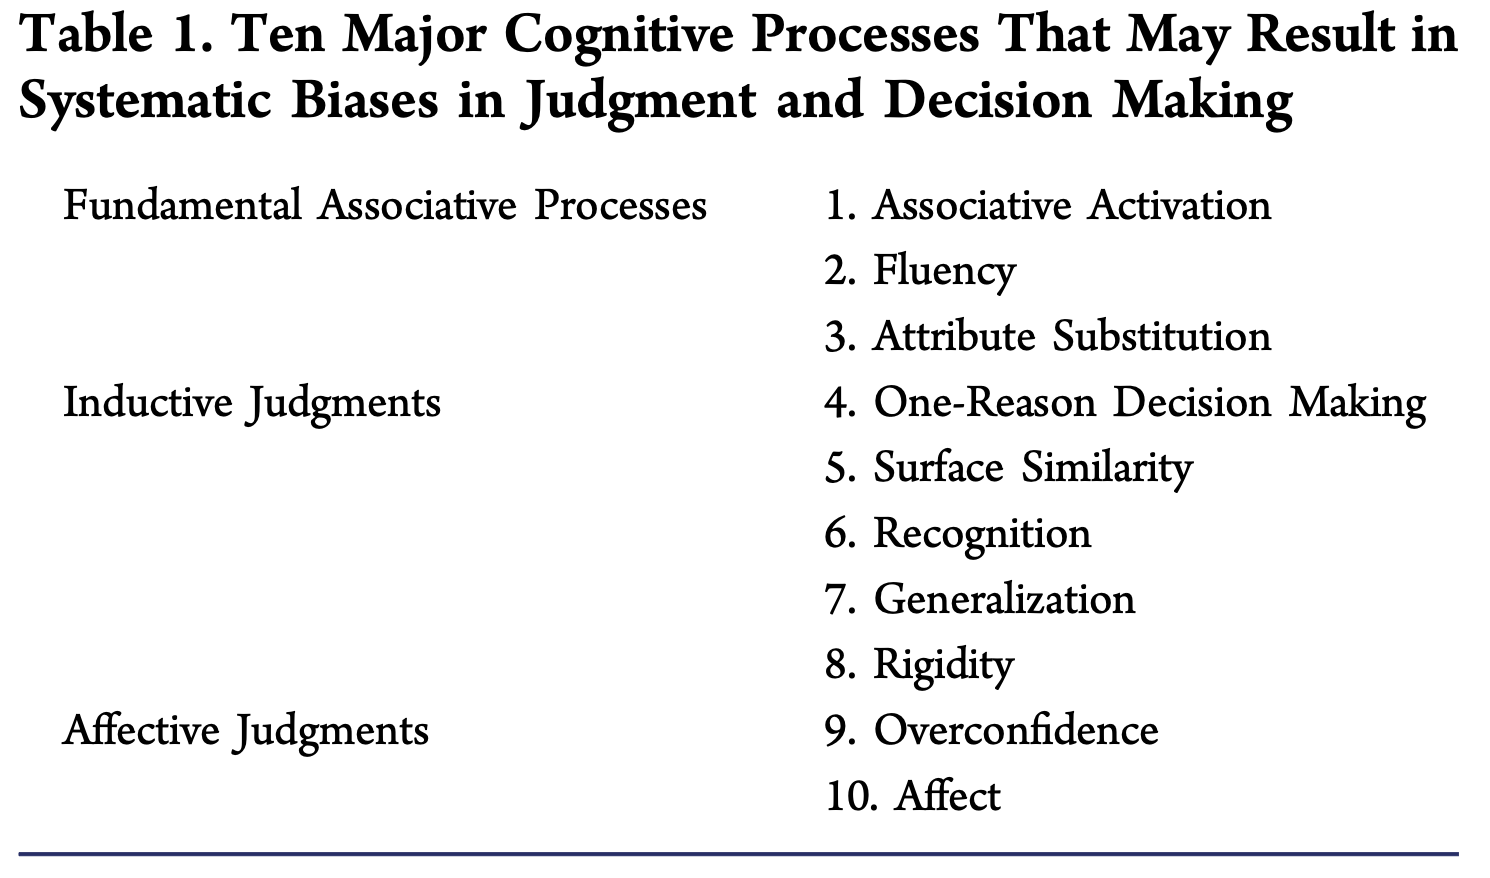
\includegraphics[width=0.9\textwidth]{pictures/systematic_biases.png}
        \caption{Deset problematických myšlenkových procesů, které brání správnému rozhodování. \cite{talanquer2014}}
        \label{fig:talanquer}
    \end{figure}{}
    

Problematice heuristických metod v oblasti především organické chemie se zabývá Nicole Graulich. Cílem její práce je identifikovat myšlenkové vzorce žáků, které by následně mohly pomoci pedagogům k efektivnějšímu vysvětlení principů organické chemie, které následně povedou k účinnému učení žáků pomocí heuristických metod výuky. \cite{graulich2010, graulich2012}\\

\section{Heuristické pokusy}

V následující kapitole bych ráda popsala několik heuristických pokusů, které mohou být zařazeny do výuky chemie. Cílem pokusu je jednoduše demonstrovat nějaký jev či přítomnost určité sloučeniny. Na základě již nabytých znalostí by měli žáci být schopni popsat, co se při daném pokusu odehrává.\\

\subsection*{Fotosyntéza a tančící hrozinky}

Popis pokusů jsou převzaty z databanky domácích pokusů Chemie hrou. \cite{chemiehrou_tancici_hrozinky, chemiehrou_fotosynteza}\\
    
    \begin{equation}
        \mathrm{CH_{3}}\mathrm{COOH} + \mathrm{NaHCO_{3}} \rightarrow \mathrm{CH_{3}}\mathrm{COOHNa} + \mathrm{H_{2}O} + \mathrm{CO_{2}}
    \end{equation}\\

    
Principem prvního pokusu, který studenti provádí je reakce hydrogenuhličitanu sodného $\mathrm{NaHCO_{3}}$ (kuchyňské jedlé sody) s kyselinou octovou $\mathrm{CH_{3}COOH}$ přítomnou v octě. Zavařovací sklenici nejprve do poloviny naplníme vodou, poté přidáme pět velkých lžic octa a přidáme několik hrozinek. Samotnou demonstraci zahájíme přidáním malé lžičky jedlé sody do naplněné sklenice s hrozinkami, směs nemícháme. Přidáním jedlé sody začne ve sklenici vývoj plynu ve formě bublinek. Žáci pozorují jak bublinky zachycené na hrozinkách nadnášejí hrozinky ke hladině a po uvolnění bublinek do okolního vzduchu hrozinky padají směrem ke dnu. \\

Pro druhý experiment si připravíme druhou zavařovací sklenici a vodní rostliny. Naplníme zavařovací sklenici vodou a přidáme do ní lžičku jedlé sody a směs zamícháme. Poté vložíme do sklenice kousek vodní rostliny tak, aby byla celá ponořená. Rostlinu osvítíme intenzivním světlem, například stolní lampičkou. V prvním okamžiku nedochází k pozorovatelným změnám ve sklenici, proto začneme s žáky objevovat výsledky prvního pokusu, který si studenti mohou jednoduše zopakovat přidáním další lžičky jedné sody do sklenice s hrozinkami. \\

Po přibližně deseti minutách by měli žáci pozorovat, jak se z listů vodní rostliny uvolňují bublinky plynu, v tomto případě se jedná o kyslík. Během dalšího výkladu srovnáme vývin obou plynů a můžeme volně přejít k chemickému principu fotosyntézy.\cite{prirodovedci_fotosynteza}\\

    \begin{equation}
        6\, \mathrm{CO_{2}} + 12\, \mathrm{H_{2}O} \rightarrow \mathrm{C_{6}H_{12}O_{6}} + 6\, \mathrm{O_{2}} + 6\, \mathrm{H_{2}O}
    \end{equation}

Pro zopakování výklady případně jako domácí úkol je možné zařadit elektronické zdroje například videa. Přehledně princip fotosyntézy popisuje "Nezkreslená věda II: Co je to fotosyntéza?" od Akademie věd ČR. \cite{nezkreslena_veda_fotosynteza}\\

V chemii existuje velká řada materiálů a pomůcek k názorným pokusům. Je asi zbytečné zde pokusy přepisovat, pouze uvedu příklady elektronických zdrojů, ze kterých je možné čerpat. Mimo tyto webové stránky lze najít mnoho závěrečných prací z různých univerzit, které jsou taktéž přístupné pro inspiraci do vlastních hodin.

    \begin{itemize}
        \item Chemie hrou - databáze domácích pokusů \cite{chemiehrou}
        \item Domácí pokusy z chemie \cite{pokusy_zsletohrad}
        \item Chemické pokusy - Studium chemie: Portál PřF UK pro podporu výuky chemie na SŠ a ZŠ \cite{chemicke_pokusy_pruk}
        \item Netradiční experimenty z organické a praktické chemie - přírodní látky, neobvyklé uspořádání a pomůcky \cite{sulcova2007}
        \item Domácí chemické pokusy \cite{domaci_chemicke_pokusy_dusova}
        \item Periodická video tabulka prvků - Návody na chemické pokusy \cite{chemicke_prvky}
    \end{itemize}

\chapter{Heuristické metody \\ve vysokoškolské pedagogice}

Tradiční výukovou formou ve vysokoškolské pedagogice je přednáška. Přednáška je řečnický útvar, jde o mluvený výklad určitého tématu. Z tohoto pohledu se přednáška skládá ze tří částí - úvodu, jádra a závěru. V úvodu řečník seznámí posluchače s daným tématem, výchovně vzdělávacím cílem a osnovou. Měly by také zaznít hlavní klíčové myšlenky, na které přednáška bude hledat odpovědi. Jádro přednášky by mělo být dále členěno do logických částí. Na závěr by mělo zaznít shrnutí podstatných informací a představení praktických přínosů. Současně by měla být představena literatura a metodické pokyny pro práci s ní. \cite{slavik2012,elergning_ujak_prednaska} \\

Mezi hlavní negativa přednášení dle S. P. Hoovera  patří nízká aktivizace studentů. Tato metoda podporuje pouhé předávání faktů, není vhodná pro dosažení cílů jako jsou utváření postojů nebo rozvoj dovedností, je minimalizováno sociální učení a je podporován koncept učitele jako poslední autority. Mimo to je obtížné přizpůsobit výklad potřebám studentů. \cite{slavik2012} Pro odklon od klasické přednášky popsané výše nahrává také fakt, že ačkoliv se jedná o vzdělávání dospělých, i ti ztrácí pozornost po přibližně dvaceti minutách výkladu, proto je třeba výklad vést dynamicky, uvolnit napětí a pozornost kladením otázek či provedením demonstrace. \cite{rohlikova2012}\\

Pokud má být vysokoškolská příprava kvalitní a vést k rozvoji osobnosti, zvyšování celkové intelektuální úrovně studentů, k osvojení vědeckých metod práce, samostatnosti a tvořivosti, je třeba využít aktivizujících metod výuky. \cite{novotna1985} Je pochopitelné, že není možné úplně nahradit přednášky jinými komplexnějšími metodami výuky, ale lze postavit přednášky tak, aby byla jejich didaktická hodnota mnohem větší. Jednou z možností je domácí příprava na další hodinu, která musí být ale nejen kontrolována, ale musí dávat smysl a být opravdu na další přednášce využita. Lze zapojit krátké demonstrace s využitím audiovizuání techniky, doplnit výklad o problémovou úlohu či heuristický rozhovor. Efektivní metodou aktivizace většího množství studentů je také hlasování či krátká diskuze v menších skupinách nad zadaným problémem.\cite{rohlikova2012}
